\section{The Comparison}
\label{sec:comparison}

\begin{figure}[t]\centering
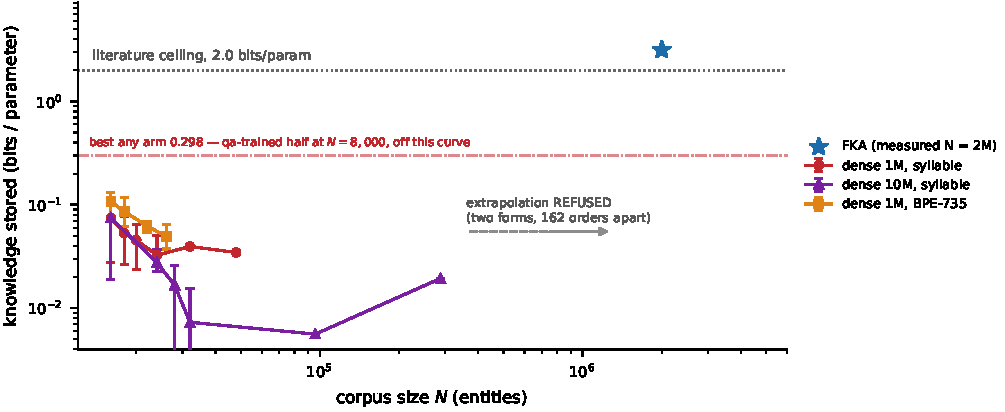
\includegraphics[width=0.85\linewidth]{figures/F1_frontier}
\caption{\textbf{Knowledge stored per parameter, against corpus size.} The dense baseline is a plain
LM trained on the same world with the fact firewall off, under the capacity literature's own recipe,
on a surface chosen to match its regime. \textbf{Every point is plotted at the $N$ it was measured
at.} No point is extrapolated --- the dense side's extrapolation to $N = 2$M was attempted and
\emph{refused}, for the reason in \S\ref{sec:refusal}. The dense side is limited by \emph{addressing},
not by bits: every arm that failed did so at under $0.19\times$ of its theoretical bit capacity, and
the best bits/parameter observed across every arm ever run is \textbf{0.298} against a ceiling of
2.0 it never approaches. \textbf{Each dense point is measured at its own $N$}, mean over seeds with
the full seed range as the interval; seed counts are not uniform and are stated per arm in
Figure~\ref{fig:dense} (cliff-bracket arms $n = 10$ at 1M and $n = 5$ at 10M, alive-side
$n = 4$--$5$, and the two largest arms at each size single-seed --- licensed by their confinement to
the dead zone, \S\ref{sec:kstar}, where every seed reads far below criterion). FKA's point carries
10 seeds. \textbf{The 0.298 reference line is not on any of these curves}: it is the
\emph{qa-trained} half at $N = 8{,}000$ in the capacity sweep, a smaller corpus than any ladder arm,
where the held-out figure is 0.2720. The best held-out figure anywhere on the ladder is 0.1322.
0.298 is quoted because it is the most generous reading available to the baseline, and it is
labelled so it cannot be read as a value at any plotted $N$.}
\label{fig:frontier}
\end{figure}

\subsection{The plot}

Figure~\ref{fig:frontier} places FKA at its measured operating point ($N = 2$M, 8M facts) and the
dense baseline at the sizes it was measured at ($N = 8{,}000$--$288{,}000$, at 1M and 10M
parameters). \textbf{The two sides are measured at different $N$, and the plot says so on its face.}

This is the same discipline that descoped the 150M dense run rather than quoting an unsaturated one,
and that M3 imposed after the stale-constant correction: a point is plotted where it was measured.

\subsection{The refusal is a result}
\label{sec:refusal}

Placing the dense point at $N = 2$M requires extrapolating $\alpha$ two orders of magnitude in $N$
and nine or more in parameters, from a measurement spanning \emph{one} order.

\begin{center}\small
\begin{tabular}{@{}p{4.6cm}p{9.4cm}@{}}
\toprule
form & parameters required for 2M discriminable keys \\
\midrule
power, $\alpha = 0.291$ & $1.3 \times 10^{13}$ \\
power, $\alpha = 0.224$ & $1.7 \times 10^{15}$ \\
power, $\alpha = 0.185$ & $1.4 \times 10^{17}$ \\
\textbf{log}, $K^* = 3{,}482\log_2 P - 52{,}120$ & $\mathbf{10^{177}}$ \\
\bottomrule
\end{tabular}
\end{center}

\medskip
\noindent Both forms pass through both measured points with \textbf{zero residual} --- two points
cannot discriminate a functional form --- and they disagree about $N = 2$M by \textbf{162 orders of
magnitude}.
% experiments/2026-08-04_frontier/plot_data.json | M5 5.146

The restraint rule asks whether the undetermined choice changes the decision. Elsewhere in this
study it did not: two candidate forms for the address-cost curve both predicted within one ladder
step and both put gate failure between 2.4M and 3.2M entities, so the disagreement was immaterial
and the agreement was the reportable fact (\S\ref{sec:fka}). \textbf{Here the choice decides
everything}, so nothing about $N = 2$M is said.

\begin{quote}
An extrapolated point carrying an honest error bar of 162 orders of magnitude is not a point. The
refusal is the stronger statement, and it is the one the plot carries.
\end{quote}

\subsection{The refusal is symmetric, and that is what makes it a refusal}
\label{sec:symmetric}

A refusal that runs in one direction only is a preference. This one runs in both, and the objection
it answers is the sharpest available against \S\ref{sec:reconc}:

\begin{quote}
\emph{You decline to extrapolate $\alpha$ to $N = 2$M, yet you conclude that the capacity
literature's regime sits below an addressing wall. Locating someone else's regime relative to a wall
is an extrapolation. Either $\alpha$ travels or your reconciliation does not.}
\end{quote}

\noindent The objection would be correct against a claim we do not make. \textbf{We do not locate the
reference's wall, and nothing in the reconciliation requires locating it.} The reconciliation is
arithmetic in params per key at \emph{our} measured points: a gap of $1.89\times$ against carriers of
$2.35\times$, one an accounting identity given their attribute count and the other measured on our
own corpus at 1M. No $\alpha$ appears in it, and no quantity is transported into their regime.

What we assert about their regime is the weaker, non-extrapolated statement: \textbf{our arms are
past a wall, theirs report no such collapse, and two measured factors account for the difference in
per-key cost without appealing to one.} Where their wall sits, whether they have one, and whether
$\alpha$ describes their scaling are all \emph{unknown to us}, and they are unknown for exactly the
reason \S\ref{sec:refusal} gives: the same two functional forms that disagree by 162 orders of
magnitude going up disagree just as violently coming down. \emph{An exponent that cannot be
extrapolated forward cannot be extrapolated backward either}, and the inference ``their regime must
therefore be past its own wall'' dies by the identical argument --- which is why we do not make it,
and why the not-quoted table (\S\ref{sec:refuse}) is the honest place for it.

\scope{This also bounds the paper's own reach in the direction that costs us. We have shown a wall
exists in \emph{our} regime and priced what crossing it does. We have not shown that dense storage
is bounded in general, that the reference's numbers are unattainable, or that any frontier model is
subject to what we measured at 1M and 10M parameters on a synthetic corpus.}

\subsection{The structural asymmetry}

Stated in its earned, mechanism-neutral form --- \emph{magnitudes only}, no claim about why.

\begin{figure}[t]\centering
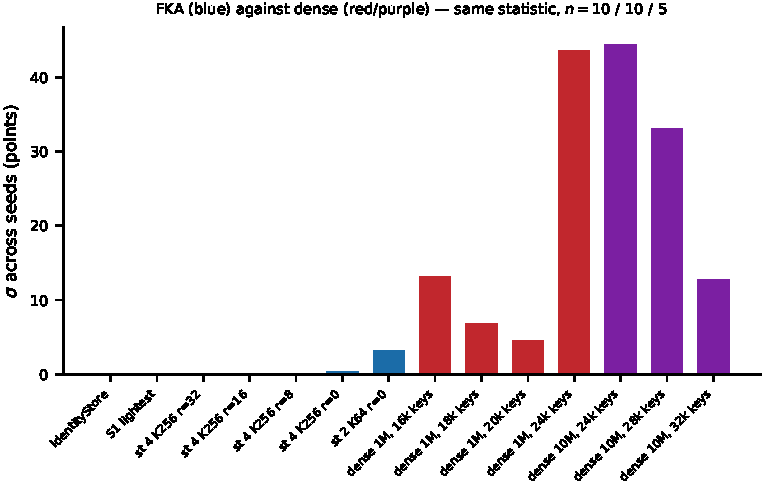
\includegraphics[width=0.80\linewidth]{figures/F7_seeds}
\caption{Seed spread, same statistic (chance-corrected recall across independent seeds at a fixed
configuration), $n = 10$ / $10$ / $5$. FKA shows $\sigma = 0.00$ at five of seven compression rungs
including its operating point.}
\label{fig:seeds}
\end{figure}

\begin{center}\small
\begin{tabular}{@{}lll@{}}
\toprule
 & at the operating point & at the transition \\
\midrule
FKA addressability & $\sigma = \mathbf{0.00}$ (five rungs) & $\sigma = \mathbf{3.20}$ \\
dense recall & $\sigma \approx 4.6$ & $\sigma = \mathbf{12.7}$--$\mathbf{44.5}$ \\
\bottomrule
\end{tabular}
\end{center}

\medskip
\noindent A factor of 4--14 at the respective transitions, and categorical at the respective
operating points. \textbf{Addressing is explicit and priced on one side} --- $2.38\log_2 N$ bits per
entity, measured, with a bounded validity horizon --- \textbf{and implicit and cliff-shaped on the
other}, growing as $P^{0.224}$ and run-stochastic at the wall.

\scope{The two seed sweeps vary different operations: FKA's varies store fitting and evaluation
sampling, the dense one varies model initialisation and training. Both are run-to-run spread at a
fixed configuration; they are not the same operation, and no mechanism is claimed on either side.
FKA's figure is at $N = 2{,}000$ against the dense side's 16{,}000--32{,}000, and the transition
rungs are not matched in depth.}

\paragraph{The convergent diagnosis.} Both tracks independently resolved a capacity question into an
addressing question. On the FKA side, compression stopped being the binding constraint once the
substrate reached 42.7$\times$ at full addressability, and the open bills became address cost and
crowding. On the dense side, bits were never the binding constraint at all: every failure occurred
below $0.19\times$ of capacity. \emph{Neither track set out to measure addressing.}
